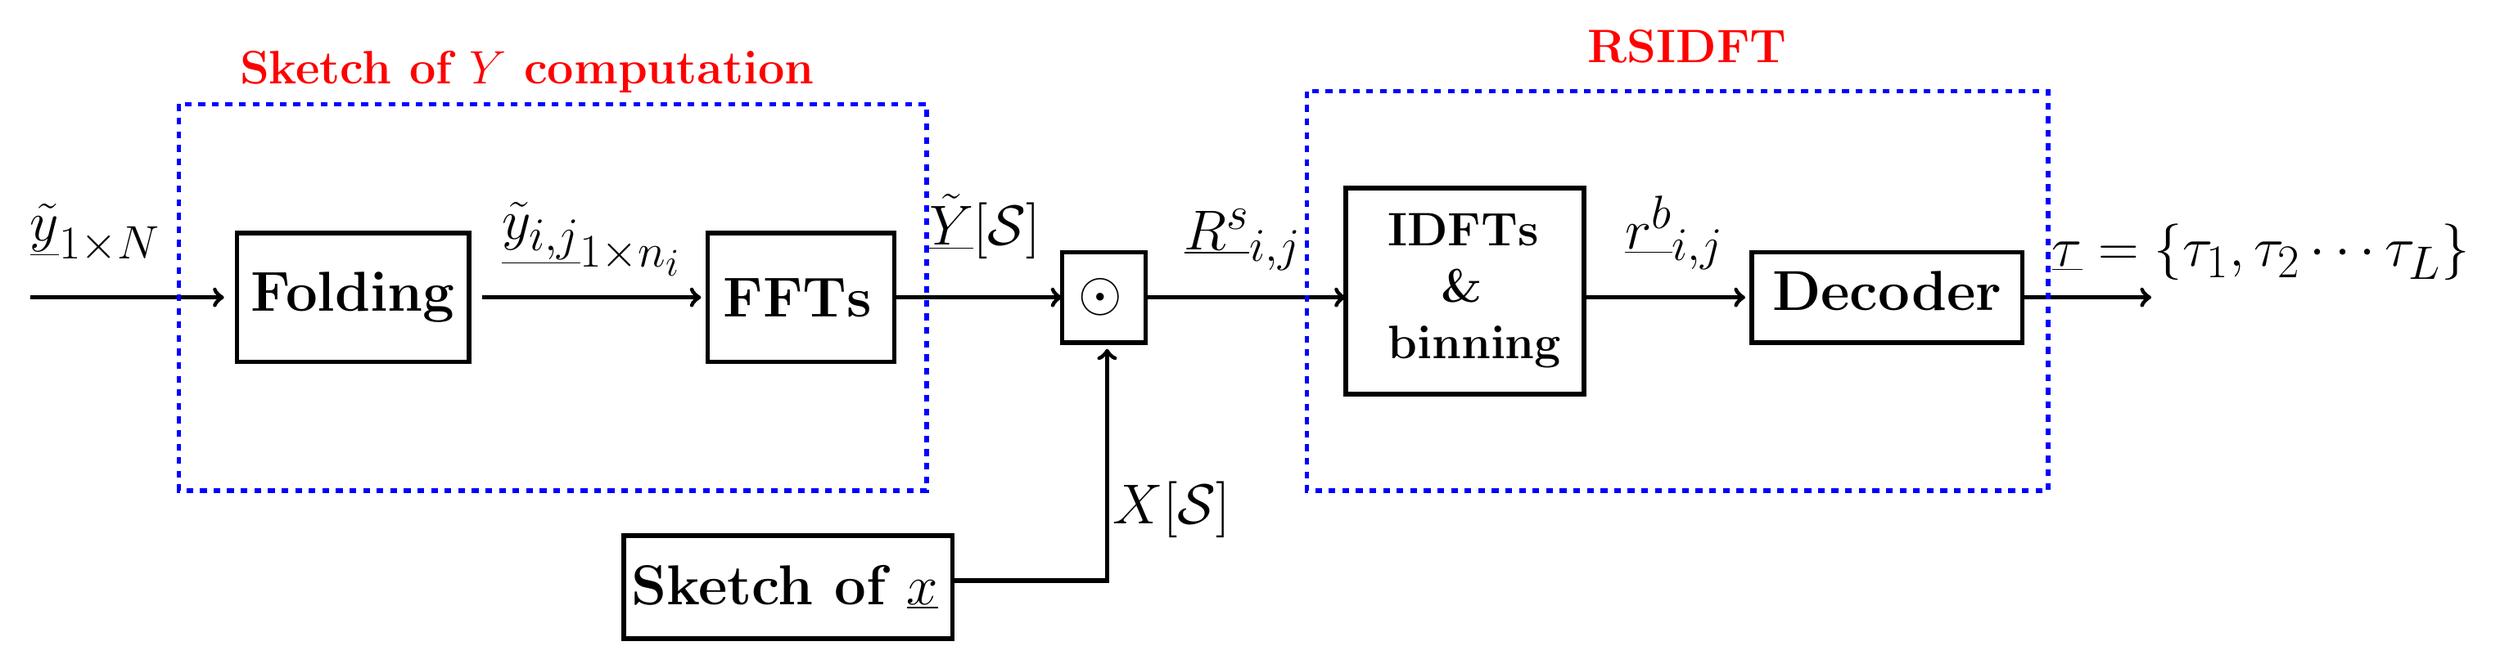
\begin{tikzpicture}

\node at (-8.7,3) { \Huge \bf  Folding};
\node at (-1.8,3) {\Huge \bf FFTs};
\node at (2.9,3) {\Huge  \bf $ \odot$};
\node [align = center] at (8.7,3.1) {\huge \bf  \begin{tabular}{l}
IDFTs \\ ~~ \& \\ binning
\end{tabular}};
\node at (-2,-1.5) { \Huge \bf Sketch of $\underline{x}$ };
\node at (15.1,3.1) {\Huge \bf  Decoder};
\draw [thick,line width =2] (-10.5,4) rectangle (-6.9,2);
\draw [thick,line width =2] (-3.2,4) rectangle (-0.3,2);
\draw [thick,line width =2] (2.3,3.7) rectangle (3.6,2.3);
\draw [thick,line width =2] (6.7,4.7) rectangle (10.4,1.5);
\draw  [thick,line width =2] (-4.5,-0.7) rectangle (0.6,-2.3);
\draw  [thick,line width =2] (13,3.7) rectangle (17.2,2.3);
\draw[->, thick, line width=2] (0.6,-1.4) -- (3,-1.4) -- (3,2.2);
\draw[->, thick, line width=2] (-6.7,3) -- (-3.3,3);
\draw[->, thick, line width=2] (-0.3,3) -- (2.3,3);
\draw [->, thick, line width=2] (3.6,3) -- (6.7,3);
\draw[->, thick, line width=2] (10.4,3) -- (12.7,3) -- (12.9,3);
\draw[->, thick, line width=2] (17.2,3) -- (19.2,3);
\draw[->, thick, line width=2] (-13.7,3) -- (-10.7,3);
\node at (-12.7,4) {\Huge$\underline{\tilde{y}}_{1 \times N}$};
\node at (-5,3.9) {\Huge$\underline{\tilde{y}_{i,j}}_{1 \times n_i}$};
\node at (11.8,4) {\Huge$\underline{r^b}_{i,j}$};
\node at (20.9,3.7) {\Huge$\underline{\tau } = \{\tau_1, \tau_2 \cdots \tau_L \}$};
\node at (4,-0.3) {\Huge $X[\mathcal{S}]$};
\node at (5.1,3.9) {\Huge $\underline{R^s}_{i,j}$};
\node at (1.1,4.1) {\Huge$\underline{\tilde{Y}}[\mathcal{S}]$};
\draw [dashed, line width =2, color=blue] (-11.4,6) rectangle (0.2,0);
\node[color= red] at (-6,6.5) {\huge \bf  Sketch of $Y$ computation};
\draw [dashed, line width =2, color=blue]  (6.1,6.2) rectangle (17.6,0);
\node [color = red] at (12,6.9) {\huge \bf RSIDFT};
\end{tikzpicture}